\documentclass[paper=a4, fontsize=11pt]{scrartcl} % A4 paper and 11pt font size
\usepackage[utf8]{inputenc}
\usepackage{listings}
\usepackage[table,xcdraw]{xcolor}
\usepackage{graphicx}
\usepackage{color}
\usepackage[italian]{babel} % English language/hyphenation
\usepackage{amsmath,amsfonts,amsthm} % Math packages
\usepackage{enumerate}
\usepackage{hyperref}
\usepackage{listings}



\usepackage{fancyhdr} % Custom headers and footers
\pagestyle{fancyplain} % Makes all pages in the document conform to the custom headers and footers
\fancyhead{} % No page header - if you want one, create it in the same way as the footers below
\fancyfoot[L]{} % Empty left footer
\fancyfoot[C]{} % Empty center footer
\fancyfoot[R]{\thepage} % Page numbering for right footer
\renewcommand{\headrulewidth}{0pt} % Remove header underlines
\renewcommand{\footrulewidth}{0pt} % Remove footer underlines
\setlength{\headheight}{13.6pt} % Customize the height of the header

\numberwithin{equation}{section} % Number equations within sections (i.e. 1.1, 1.2, 2.1, 2.2 instead of 1, 2, 3, 4)
\numberwithin{figure}{section} % Number figures within sections (i.e. 1.1, 1.2, 2.1, 2.2 instead of 1, 2, 3, 4)
\numberwithin{table}{section} % Number tables within sections (i.e. 1.1, 1.2, 2.1, 2.2 instead of 1, 2, 3, 4)

\setlength\parindent{0pt} % Removes all indentation from paragraphs - comment this line for an assignment with lots of text

\graphicspath{{img/}}

%----------------------------------------------------------------------------------------
%	TITLE SECTION
%----------------------------------------------------------------------------------------

\newcommand{\horrule}[1]{\rule{\linewidth}{#1}} % Create horizontal rule command with 1 argument of height

\title{	
\normalfont \normalsize 
\textsc{Sistemi Distribuiti, Università degli studi di Udine} \\ [25pt] % Your university, school and/or department name(s)
\horrule{0.5pt} \\[0.4cm] % Thin top horizontal rule
\huge Distribute a soft real-time 3d multiplayer game% The assignment title
\horrule{2pt} \\[0.5cm] % Thick bottom horizontal rule
}

\author{Boubakr Injarn mat. 112194\\Alexandru Pruteanu mat. 111021} % Your name

\date{\normalsize\today} % Today's date or a custom date

\begin{document}

\maketitle % Print the title
\newpage
\tableofcontents
\listoffigures
\newpage
\textbf{\abstractname}

Il seguente progetto consiste nell'implementazione di un gioco in prima persona, real-time e distribuito. Lo scopo principale è di realizzare l'applicazione tenendo conto soprattutto di aspetti che riguardano, in particolare, la comunicazione (cioè affidabilità, consistenza e disponibilità del servizio).



\section{Analisi dei requisiti}


\subsection{Scopo}
Permettere a uno o più utenti di poter comandare una nave spaziale al fine di difendere il pianeta terra dalla minaccia degli asteroidi. Nel secondo caso, ogni utente deve vedere singolarmente le azioni degli altri utenti e lo stato globale del sistema deve essere uguale per tutti.


\subsection{Requisiti}
\begin{enumerate}
\item Il sistema deve dare la massima trasparenza all'utente per quanto riguarda la comunicazione tra i vari moduli. L'utente deve poter avviare l'applicazione (il client) e poter iniziare a giocare la partita.
\end{enumerate}


\subsection{Casi d'uso}
Sotto in figura ? sono illustrati i casi d'uso più rilevanti, le interface utente e il
diagramma di flusso dei messaggi che vengono scambiato fra il client e il server.


\subsubsection{Multiplayer, creazione di una nuova room}

Sotto sono in figura ? viene illustrato l'interfaccia utente:

\begin{figure}[h]
\centering
\includegraphics[width=\textwidth]{MultiplayerCreateRoomUC}
\caption{Create Room in modalità Multiplayer}
\label{CreateRoomUC}
\end{figure}

Sotto in figura ? si possono vedere i messaggi scambiati fra il client e il server:

\begin{figure}[h]
\centering
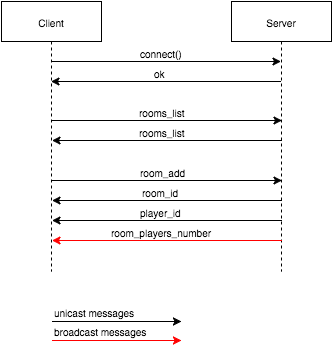
\includegraphics[width=\textwidth]{MultiplayerCreateRoom}
\caption{Create Room in modalità Multiplayer}
\label{CreateRoom}
\end{figure}


\subsubsection{Multiplayer, entrata in una room}
Sotto sono in figura ? viene illustrato l'interfaccia utente:

\begin{figure}[h]
\centering
\includegraphics[width=\textwidth]{MultiplayerJoinRoomUC}
\caption{Create Room in modalità Multiplayer}
\label{CreateRoomUC}
\end{figure}

Sotto in figura ? si possono vedere i messaggi scambiati fra il client e il server:

\begin{figure}[h]
\centering
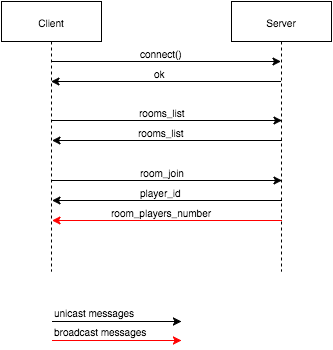
\includegraphics[width=\textwidth]{MultiplayerJoinRoom}
\caption{Create Room in modalità Multiplayer}
\label{CreateRoom}
\end{figure}

\section{Architettura e Design}
\textcolor{red}{DA INTEGRARE CON QUANTO GIA' PRESENTE SU GIT}

In figura \ref{GenArc} è possibile osservare lo schema dell'architettura generale del sistema implementato. Le componenti principali che andremo poi a descrivere sono rappresentate dal client e dal server. Come si osserva, tra questi due vi è un canale full-duplex rappresentato, nel nostro caso, da una connessione TCP (protocollo WebSocket). E' possibile inoltre osservare che i client non comunicano tra di loro in maniera diretta ma attraverso i server, i quali invece comunicano tra loro al fine di replicare le informazioni (i vari stati di gioco), distribuire il carico di lavoro (permettendo quindi una maggiore scalabilità) e garantire una certa disponibilità.

Per permettere la modalità di gioco multiplayer viene utilizzato il protocollo WebSocket, questo perchè il gioco viene eseguito all'interno del browser, il protocollo WebSocket funziona sopra HTTP con communicazione assincorna che posono avvenire concorrente. Siccome il browser non può ricevere una connessione, ma solo inizializzarla, connessione fra più client (p2p) non è possibile (attualmente un nuovo protocollo WebRTC si sta diffondendo per appunto permettere architetture di tipo p2p, purtroppo è una tecnologia ancora troppo giovane).


\begin{figure}[h]
\centering
\includegraphics[width=\textwidth]{GeneralArchitecture}
\caption{Architettura generale del sistema}
\label{GenArc}
\end{figure}

In figura \ref{GenArc} i client non sono altri che dei browser con supporto per WebGL e WebSocket. All'inizio un client (browser) esegue una richiesta al DNS per ricevere l0indirizzo del WebServer, il DNS è anche responsabile del load balancing. Una volta ricevuta la risposta dal DNS con l'indirizzo di uno dei WebServer il client fa una richiesta e riceve tutti gli asset del gioco (js, imagini, css, ...). Il WebServer e solo responsabile per fornire gli asset del gioco, ne di più ne di meno. Infine il client si connete ad uno dei server del gioco (Erlang) e decide di creare una nuova stanza o entrare in una esistente. I server sono scritti nel linguaggio Erlang e con lo scopo primario di essere fault tolerant e distribuiti.

\begin{figure}[h]
\centering
\includegraphics[width=\textwidth]{CAP}
\caption{teorema di Brewer}
\label{CAP}
\end{figure}

In un mondo ideale sarebbe molto bello avere sia Availability che Consistency allo stesso tempo.
In un mondo reale purtroppo cio è impossibile, ed è questo che afferma il teorema di Brewer (CAP Theorem), puoi avere solo 2 cose alla volta (che sono: CP, AP oppure AC), teoriticamente parlando una soluzione AC potrebbe essere possibile, ma purtroppo noi tutti sappiamo che non esiste hardware e reti al mondo che non falliscono mai.
Per il gioco e sistema in analisi sis è optato per un'architettura AP (cioè Availability e Partition tolerance). In un gioco soft real-time è molto più importante un sistema disponibile che consistente (almeno cosi è per questo gioco). In caso di fallimenti è preferibile perdere consistenza (risincronizzare e risolvere conflitti più avanti) e guadagnare disponibilità continua del servizio.

Di seguito vengono elencati i messaggi scambiati fra il client e il server. Per la rappresentazione esterna dei dati viene utilizzato il formato JSON. Lo stesso messaggio ricevuto dal client o dal server può avere funzionalità diverse, ad esempio inizialmente il client manda un messaggio room\_list che server a chiedere al server la lista delle room disponibili, di seguito il server risponde sempre con un messaggio room\_list accompagnato dai dati. Come si può osservare il messaggio è lo stesso ma ha semantica diversa se ricevuto dal client oppure dal server, il tutto e per evitare messaggi duplicati, come add esempio: room\_list\_get, room\_list\_set, ....

Sotto sono elencati i messaggi mandati dal client al server:
\begin{itemize}
\item rooms\_list \textit{(richiesta per la lista delle room disponibili)}
\item room\_join \textit{(richiesta per entrare in una room)}
\item room\_add (richiesta per creare una nuova room)
\item action\_earth\_collision (segnalare che c'è stata una collisione con un'asteroide)
\item ship\_position (richiesta della posizione della navicella degli altri giocatori)
\item game\_master\_asteroids\_position (richiesta per la posizione degli asteroidi prima di entrare nel gioco, da un client master)
\item game\_ship\_position \textit{(richiesta per la posizione delle navicelle nel gioco)}
\item action\_ship\_move \textit{(segnalare al server e altri client che la navicella si sta spostando)}
\item action\_ship\_shot \textit{(segnalare al server e altri client che la navicella ha sparato)}
\item ping \textit{(messaggio di heartbeat, per dire al server che si è ancora in ascolto e di non chiudere la connessione con il client)}
\end{itemize}


Sotto sono elencati i messaggi mandati dal server al client:
\begin{itemize}
\item room\_list (restituisce un elenco delle room disponibili)
\end{itemize}

\subsection{Cowboy 2.0}
Come server HTTP è stato deciso di utilizzare la libreria \href{https://github.com/ninenines/cowboy}{Cowboy} interamente scritta in Erlang poiché fornisce un ottimo supporto per le WebSocket (tutte le versioni sia standard che non definitive), modello su cui è basato il progetto.

Uno dei punti di forza di Cowboy sicuramente è la semplicità del codice. I 3 moduli principali che verranno descritti nel dettaglio nella sezione successiva sono di facile comprensione e composti ciascuno da poche righe di codice di base ben documentato, da arricchire, ovviamente, secondo le esigenze del programmatore.

\subsection{Architettura client}
Per entrare maggiormente ne dettaglio, in figura \ref{ClientArc} è possibile osservare l'architettura del singolo client.

[...]

\begin{figure}[h]
\centering
\includegraphics[width=\textwidth]{ClientArchitecture}
\caption{Architettura del client}
\label{ClientArc}
\end{figure}

\subsection{Architettura server}
In figura \ref{ServerArc} possiamo invece osservare l'architettura che è stata implementata per il server.

\begin{figure}[h]
\centering
\includegraphics[width=\textwidth]{ServerArchitecture}
\caption{Architettura generale del server}
\label{ServerArc}
\end{figure}

Il server è interamente scritto in Erlang e la libreria principale utilizzata, oltre Cowboy è \href{https://github.com/davisp/jiffy}{text}{Jiffi}. Vi sono in tutto 7 moduli di cui 3 in particolare per la gestione della \textit{websocket} di seguito descritti.
\subsubsection{websocket\_app}
Il modulo \texttt{websocket\_app} è responsabile della configurazione e dell'avvio del processo server (nel nostro caso un server Cowoby). Il modulo risponde con la medesima configurazione ad ogni richiesta.
Di seguito è possibile osservare la parte di codice dove viene indicato di avviare un server in ascolto sulla porta \texttt{8888} con protocollo \texttt{http} e inoltrare le richieste al modulo \texttt{ws\_handler}.

\lstset{language=erlang}
\begin{lstlisting}
start(_Type, _Args) ->
  Dispatch = cowboy_router:compile([
    {'_', [{"/websocket/", ws_handler, []}]}
  ]),
  {ok, _} = cowboy:start_clear(http, 100, [{port, 8888}], #{
    env => #{dispatch => Dispatch}
  }),
  websocket_sup:start_link().
\end{lstlisting}

\subsubsection{websocket\_sup}
\texttt{websocket\_sup} funge da modulo supervisore (se ad esempio si blocca Cowboy, si occupa di riavviare il processo).
\subsubsection{ws\_handler}
\texttt{ws\_handler} è il modulo principale che si occupa della gestione di tutte le richieste/risposte alla/dalla websocket. Tutte le richieste che arrivano dall'esterno (nel nostro caso dalle operazioni di \texttt{send()} dei vari client) passano per questo modulo attraverso la funzione \texttt{websocket\_handle({text, Msg}, Req, State)} e sono del tipo: \texttt{[evento,dato]} dove \texttt{evento} indica l'azione compiuta dal client (ad esempio per indicare che la nave spaziale si sta spostando) mentre \texttt{dato} contiene gli eventuali dati da trasmettere insieme all'evento (ad esempio la direzione verso la quale la nave si sta spostando), può assumere valore \texttt{null}.
\begin{lstlisting}
% Receive/External message Handler
% Client that send messages to the server
websocket_handle({text, Msg}, Req, State) ->
  % The receiving message Msg is of type <<"[\"event\",data]">>
  [Event, Data] = jiffy:decode(Msg),
  case binary_to_list(Event) of
    "rooms_list" ->
      global_rooms_state ! {rooms_list, self()},
      reply_ok(Req, State);
    "room_join" ->
      Player = player:start(self()),
      PlayerId = uuid:generate(),
	  .
	  .
	  .
    "ship_shoot" ->
      global_rooms_state ! {ship_shoot, Data, State#state.room_id},
      reply_ok(Req, State);
    Unknown ->
      erlang:display("Warning: websocket_handle can not handle event:"),
      reply_ok(Req, State)
  end;
websocket_handle(_Data, Req, State) ->
  {ok, Req, State}.
\end{lstlisting}
In particolare, come si può osservare dal codice sopra, se una istanza di \texttt{Msg} collima con una delle clausole del \texttt{case} allora viene eseguita l'operazione corrispondente.

Il presente modulo si occupa anche di rispondere alle richieste inoltrate dai client qualora fosse possibile. La funzione preposta per lo scopo è \texttt{websocket\_info({Event, Data}, Req, State)}.
\begin{lstlisting}
% Send/Internal message Handler
% Server that send messages to the client
websocket_info({Event, Data}, Req, State) ->
  case Event of
    player_id ->
      reply([<<"player_id">>, Data], Req, State);
    rooms_list ->
      reply([<<"rooms_list">>, Data], Req, State);
    .
    .
    .
    Unknown ->
      erlang:display("Warning: websocket_info can not handle event:"),
      erlang:display(Unknown),
      reply_ok(Req, State)
  end.
\end{lstlisting}
Come nel caso precedente, anche la risposta al client è della forma \texttt{[evento,dato]}. Come varrà descritto successivamente, \texttt{websocket\_info/3} viene invocata da Cowboy ogni qualvolta il modulo riceva un messaggio Erlang.
\subsubsection{Moduli Erlang gestione logica di gioco e scambio messaggi}
I restanti 4 moduli servono principalmente a gestire la logica del gioco e quindi mantenere uno scambio messaggio consistente. Come si può osservare in figura \ref{ServerArc}, lo scambio messaggi avviene solo ed esclusivamente tra i moduli stessi e \texttt{ws\_handler} (eccezion fatta per \texttt{config}), questi messaggi, come precedentemente affermato, una volta inoltrati al modulo \texttt{ws\_handler} vengono passati direttamente alla funzione \texttt{websocket\_info/3}.
\begin{itemize}
\item \texttt{config}: modulo di configurazione iniziale del gioco
\item \texttt{global\_room\_state}: modulo che contiene lo stato globale del gioco, in particolare la lista di tutte le eventuali \textit{room} attive. Nella sezione successiva verrà descritto dettagliatamente come avvengono le operazioni di creazione e join nella \textit{room}, per ora è sufficiente sapere che ogni player può fare parte di una e una sola \textit{room} in modo quindi da permettere il multicast dei messaggi (visto a livello di stato globale) oppure broadcast (visto a livello di singola room).

Il modulo \texttt{ws\_handler} si occupa di inviare messaggi Erlang al modulo descritto che resta in ascolto con \texttt{handle\_info/2} ed in caso di matching esegue le operazioni indicate (si rimanda alla visione del codice per maggiori dettagli).

In generale, il modulo \texttt{global\_rooms\_state} si occupa di creare/eliminare le room di gioco, di aggiungere/rimuovere i player che ne fanno richiesta nella varie room e di smistare i messaggi a queste ultime e/o direttamente ai player, in funzione dell'operazione da eseguire.
\item \texttt{room}: modulo che tiene traccia dei player iscritti e dello stato della singola room (posizione navi spaziali, valore della vita, posizione asteroidi, etc\dots).
La funzione \texttt{loop/1} rimane in ascolto di eventuali messaggi ed in generale si occupa di mantenere lo stato di gioco tra gli iscritti alla room (attraverso l'inoltro in broadcast di specifici messaggi).
\item \texttt{player}: modulo che tiene traccia dell'\texttt{id} del player. Il suo scopo principale è inoltrare eventuali messaggi che giungono dai moduli per la gestione della logica del gioco alla funzione \texttt{websocket\_info} del modulo \texttt{ws\_handler}.
\end{itemize}


\section{Documentazione tecnica}
\begin{figure}[h]
\centering
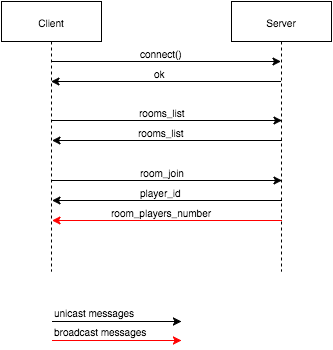
\includegraphics[width=\textwidth]{MultiplayerJoinRoom}
\caption{Join Room in modalità Multiplayer}
\label{JoinRoom}
\end{figure}

\section{Documentazione tecnica}
\begin{figure}[h]
\centering
\includegraphics[width=\textwidth]{MultiplayerJoinRoomUC}
\caption{Join Room in modalità Multiplayer}
\label{JoinRoomUC}
\end{figure}

\section{Utente finale}

\end{document}